% Chapter Template

\chapter{Empirical Study} % Main chapter title

\label{Chapter4} % Change X to a consecutive number; for referencing this chapter elsewhere, use \ref{ChapterX}

%----------------------------------------------------------------------------------------
%	SECTION 1
%----------------------------------------------------------------------------------------
\section{Study Design}\label{sec:studydesign}

This paper aims to provide information about some of the most used automatic exploration tools for android applications inside the industry and the academy. This information is going to be useful for developers and researchers when they face a decision-making situation related to the selection of the right exploration tool that fits their needs. In consequence, an empirical study was designed and will provide answers for the following research questions: 

\begin{itemize}

\item RQ-1 What tool reaches the highest accumulated method coverage?
\item RQ-2 What tool finds the largest number of failures during one exploration?
\item RQ-3 what tool has the top average value of errors found across different apps during all the explorations?
\end{itemize}

\section{Context of the Study}

To answer the research questions, 11 applications were selected to be executed. The list of selected apps can be seen in Figure.\ref{tab:apps}. This set is a subset of a set of open source applications widely used by  The Software Design Lab for other studies and tests. Every APK in the subset should be successfully instrumented by InstruAPK, it should compile without any problem after instrumentation and it should be launched in an emulator without any issue after the instrumentation process.

Equally important, four exploration tools were selected, two from the industry and two from the academic side. The first tool is Firebase Test Lab (Section \ref{sec:testlab}). It was selected for being widely used in industry and for also being a Google product. The second one, Monkey \footnote{https://developer.android.com/studio/test/monkey}, was selected as a baseline because it is the state-of-the-art and practice tool for inputs generation; it is by default included in the Android SDK Tools. The third one, Droidbot (Section \ref{sec:droidbot}), was selected from the academic side. Droidbot has been a point of study for many pieces of research. Many other tools have based their functionality on this tool. The last one is RIP (Section \ref{sec:rip}). It was selected for being of special interest for us. It is our exploration tool, and it is currently an active project inside the Software Design Lab at the University of Los Andes. 

Each tool was executed ten times per application and with a maximum time of 30 minutes. The number of executions and the maximum time was arbitrary decisions that were made because of time limitations for the study. During the study, we noticed that most of the tools ended the exploration or reached their maximum coverage within the first 15 minutes. That means that the maximum exploration time was more than enough in almost all cases. 

The same emulator was used for all the exploration tools, except for Firebase Test Lab because this tool offers its own set of emulators. In all the cases a Pixel 2 XL was used, but in the case of Monkey, Droidbot and RIP there was more control over the device specifications. For the last-mentioned tools, the specifications of the emulator used within the experiment are Google APIs Intel Atom (x86), API level 27, SD card size of 512MB, and RAM size of 4096MB. The specifications are unknown for the case of Test Lab.

\begin{table}[t]
	\centering
	\caption{Applications used for the study} \label{tab:apps}
	\resizebox{\textwidth}{!}{
		\begin{tabular}{c c c c}
			App ID & Package Name & \# Methods Reported by APKAnalyzer & \# Methods Instrumented by InstruAPK\\
			\hline
			1 & appinventor.ai\_nels0n0s0ri0.MiRutina & 61993 & 9351\\
			2 & com.evancharlton.mileage & 4000 & 1162\\
			3 & com.fsck.k9 & 18799 & 7003\\
			4 & com.ichi2.anki & 32370 & 2209\\
			5 & com.workingagenda.devinettes & 19274 & 66 \\
			6 & de.vanitasvitae.enigmandroid & 13083 & 574 \\
			7 & info.guardianproject.ripple & 19429 & 100 \\
			8 & org.connectbot & 20606 & 1145\\
			9 & org.gnucash.android & 75473 & 504\\
			10 & org.libreoffice.impressremote & 14691 & 649\\
			11 & org.lumicall.android & 45784 & 540\\
			\hline
		\end{tabular}
	}
\end{table}

Finally, the workflow specified in section \ref{sec:generalApproach} was followed for each application in table \ref{tab:apps} by using the aforementioned exploration tools. 

\section{Results}\label{sec:results}

\subsection{Method Coverage Results}\label{sec:coverageResults}

As mentioned before, some explorations ended before the max execution time allowed (30 minutes) giving no data for the upcoming seconds. To solve those scenarios, the coverage reached by the tool at the moment when the exploration end was kept the same until completing the total time. Once this has been done, the results are comparable second by second.

As a result of the instrumentation made by InstruAPK, the timestamp of every called method is known, thus, the coverage reached by a tool in a specific second can be calculated. The aforementioned information was used to calculate the average accumulated method coverage reached for every tool across the 11 analysed apps. Such results are presented in figure \ref{fig:averageCoverageInstruAPK} and figure \ref{fig:averageCoverageAPKAnalyzer}. The data were calculated as follow:

Let's take $A$ as the set of applications; $N$ as the number of explorations; $t$ as time in seconds (for this study $0<t<1800$, and T as the exploration tool, then we have:

\begin{align}
  g(a_{T,t}) &= \frac{\sum_{i=1}^{n} Coverage(T,t,a)}{N}\label{eq:g} 
\end{align}
Where $Coverage(T,t,a)$ is the instantaneous coverage of tool T in second t for the application a. Which means, the new methods called by tool T in second t.
\begin{align}
f(T_t) &= \frac{\sum_{a \in A} g(a_{T,t})}{|A|} \label{eq:f}
\end{align}
\begin{align}
H(T_t)=\begin{cases}
		H(T_{t-1})& \text{if the exploration has end},\\ 
		f(T_t)+H(T_{t-1})& \text{if still exploring},\\
		f(T_0)& \text{if $t = 0$}.\label{eq:h}
	\end{cases}
\end{align}
Thus, equation \ref{eq:g} is the average coverage of tool T for application a in time t; equation \ref{eq:f} is the average exploration of tool T in time t; and, \ref{eq:h} is what is called \textit{progressive coverage} of tool T in time t. 

Thus, equation \ref{eq:h} is what is shown in figures \ref{fig:averageCoverageInstruAPK} and \ref{fig:averageCoverageAPKAnalyzer}. For coverage in figure \ref{fig:averageCoverageInstruAPK}, equation \ref{eq:g} was calculated using the number of instrumented methods by InstruAPK and for figure \ref{fig:averageCoverageAPKAnalyzer} the number of methods reported by APKAnalyzer. The curves have the same behaviour, as expected, but in Figure \ref{fig:averageCoverageAPKAnalyzer} gap between tools is more visible.

Additionally, for every execution the called methods are stored, every method has a unique id that was given during the instrumentation. Thus, after the 10 executions of an application, every execution result could be analysed searching for the methods that have been called neither during previous explorations nor during the current one. Therefore, the number of unique methods called for one application during all 10 explorations can be obtained. That is what is named as \textit{achieved coverage} and can be seen in figure \ref{fig:boxplotAccumulated}. The coverage presented in figure \ref{fig:boxplotAccumulated} was calculated only by using the number of instrumented methods by InstruAPK. 

\begin{figure}[h]
\centering
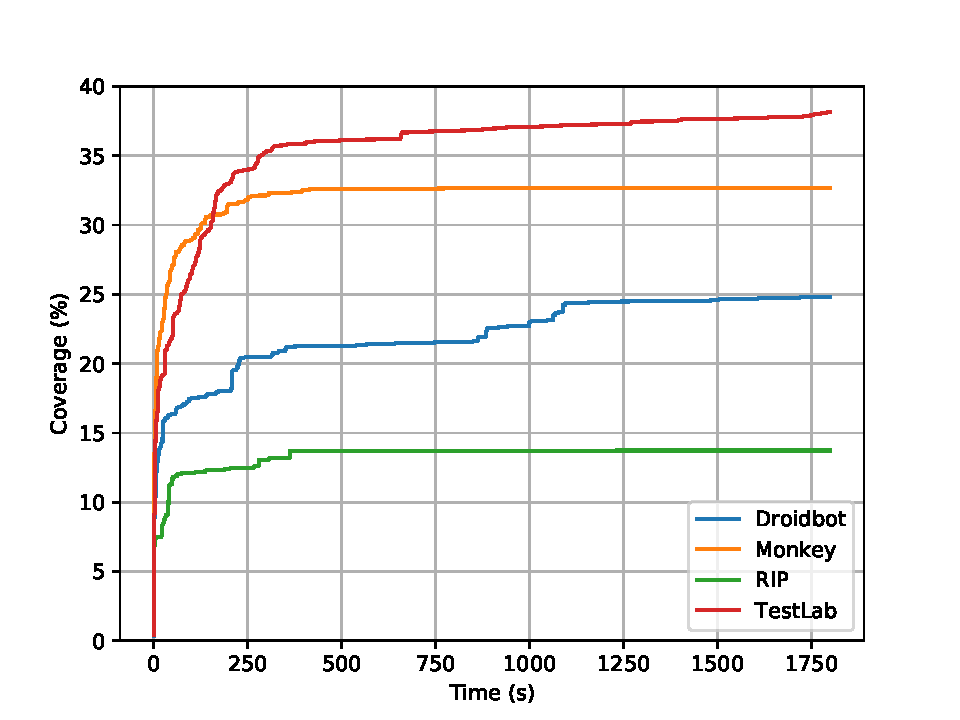
\includegraphics[width=0.8\textwidth]{../Figures/averageCoverageInstruAPK.pdf}
\caption{Average Progressive Method Coverage by Tool According to the Number of Instrumented Methods Reported by InstruAPK}\label{fig:averageCoverageInstruAPK}
\end{figure}

\begin{figure}[h]
\centering
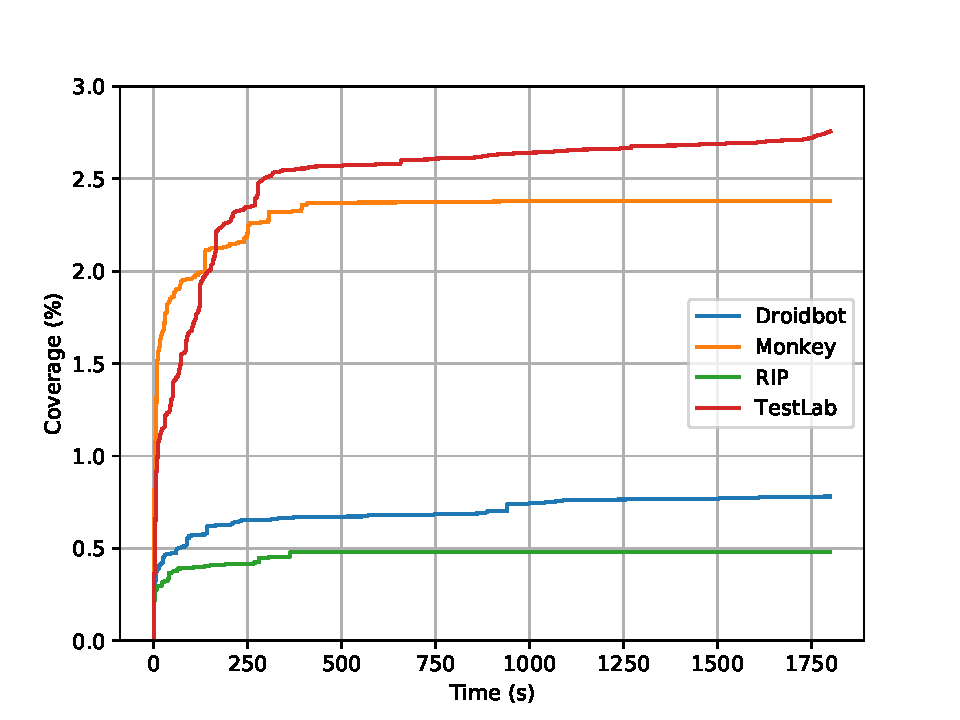
\includegraphics[width=0.8\textwidth]{../Figures/averageCoverageAPKAnalyzer.pdf}
\caption{Average Progressive Method Coverage by Tool According to the Number of Methods Reported by APKAnalyzer}\label{fig:averageCoverageAPKAnalyzer}
\end{figure}

\begin{figure}[h]
\centering
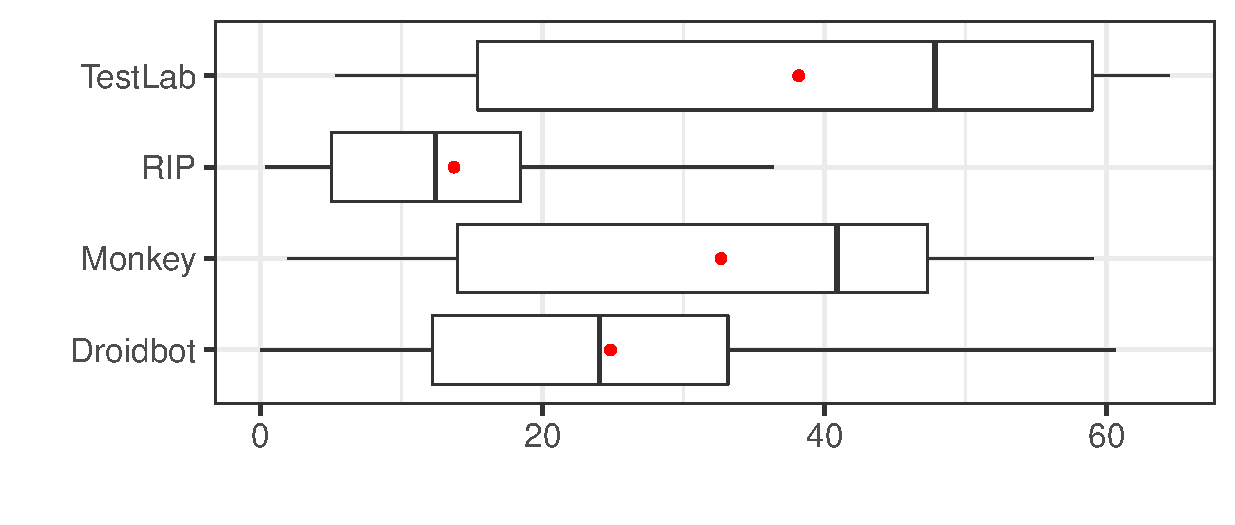
\includegraphics[width=0.8\textwidth]{../Figures/boxplotAccumulated.pdf}
\caption{Coverage Achieved by Tool}\label{fig:boxplotAccumulated}
\end{figure}


Hence, RQ-1 was responded using graphs \ref{fig:averageCoverageInstruAPK}, \ref{fig:averageCoverageAPKAnalyzer}, and \ref{fig:boxplotAccumulated}. Firebase Test Lab is the tool with the highest progressive average method coverage reached. Surprisingly, followed by Monkey, even when Monkey has no complex architecture nor exploration strategy. In the case of achieved coverage, Firebase Test Lab keeps the lead with the highest values, but now Droidbot is the tool in second place. Nevertheless, the results for Droidbot are very fluctuating, making again Monkey, the second tool with the second-best results. 

As can be seen, the dot for every tool in figure \ref{fig:boxplotAccumulated} are the max values reached in figure \ref{fig:averageCoverageInstruAPK}. So, the last graph mentioned will be the description of how each tool reached its value through time.

\subsection{Error Results}\label{sec:errorResults}

Thanks to CoverageAnalyzer, it is possible to establish the number of error traces found by an exploration tool. As explained before, CA analyses the logcat and extracts the error traces and filter them using the package name of the app under analysis. That is how the results for 
figure \ref{fig:maxerrors} and figure \ref{fig:averagaerrors} were obtained. The first graph shows only the top value found after manually analysing the results for every exploration, and the second one represents the average number of errors found across all the executions.
 

\begin{figure}[h]
\centering
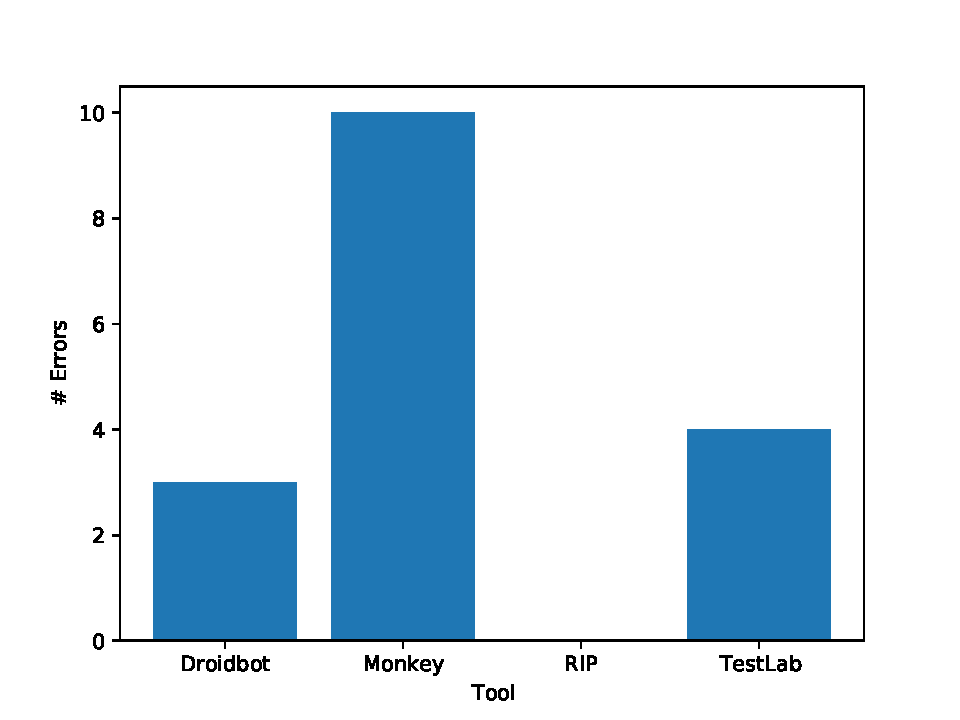
\includegraphics[width=0.8\textwidth]{../Figures/maxErrors.pdf}
\caption{Maximum Number of Errors Found by Tool in One Exploration}\label{fig:maxerrors}
\end{figure}

\begin{figure}[h]
\centering
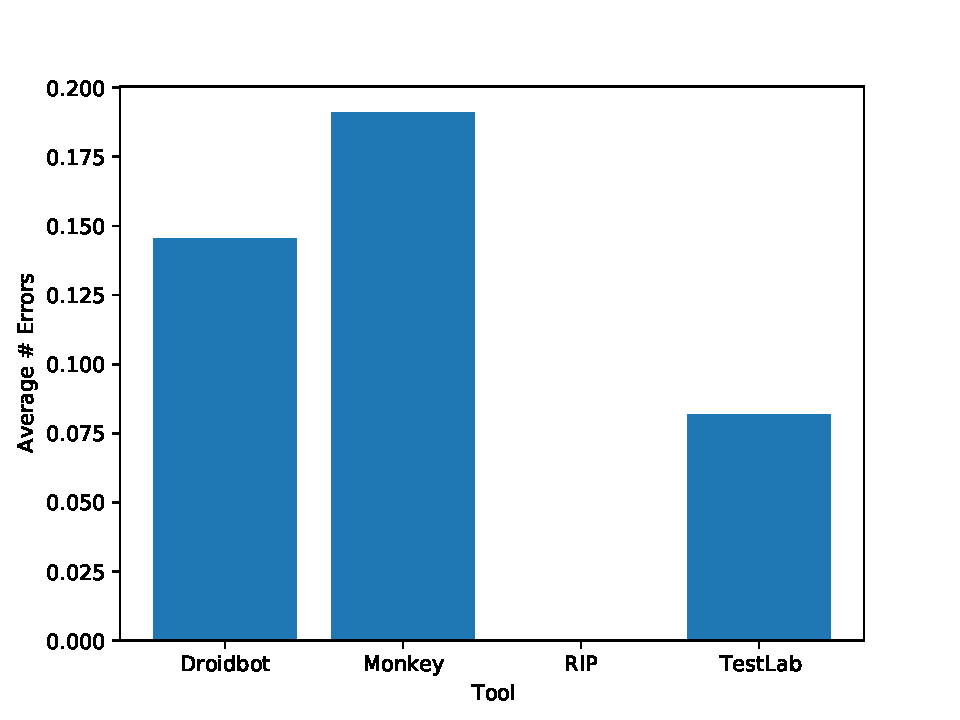
\includegraphics[width=0.8\textwidth]{../Figures/averageErrors.pdf}
\caption{Average Number of Errors Found by Tool During all the explorations}\label{fig:averagaerrors}
\end{figure}

Thus, Monkey is the tool with the top number of failures found during one exploration (RQ-2), as well as the one with the highest average errors found during all explorations (RQ-3).